The package is organized in three main steps, the peak caller in section \ref{sec:descan2peakcall}, the filtering and alignment of the peaks in section \ref{sec:descan2filtering} and the peak counting described in section \ref{sec:descan2peakcounts}.

Furthermore, it offers some additional features as described in \ref{sec:descan2addfeat}.


\begin{figure}[H]
\centering
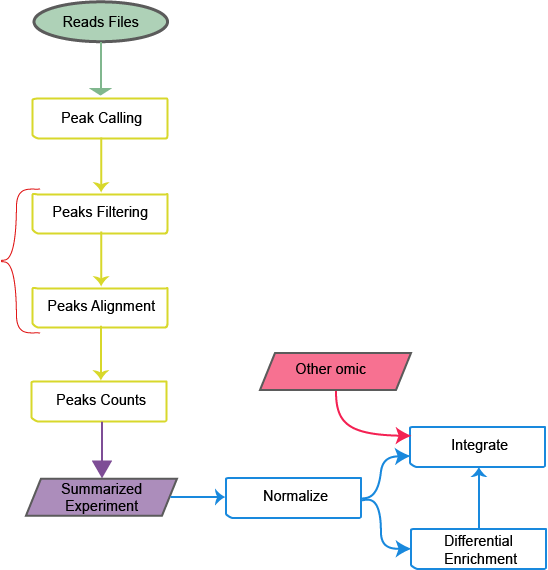
\includegraphics[width=8cm, keepaspectratio]{img/descan2/flow.png}
\caption[DEScan2 workflow]{A differential enrichement flow representation. \gls{descan} steps are highlighed in yellow.}
\label{fig:descan2flow}
\end{figure}
